\documentclass[tikz,border=3.14pt]{standalone}
\usetikzlibrary{3d,decorations.text,shapes.arrows,positioning,fit,backgrounds,arrows}
% from https://tex.stackexchange.com/a/52856/121799
\tikzset{circle dotted/.style={dash pattern=on .05mm off 2mm,
                                         line cap=round}}
\begin{document}

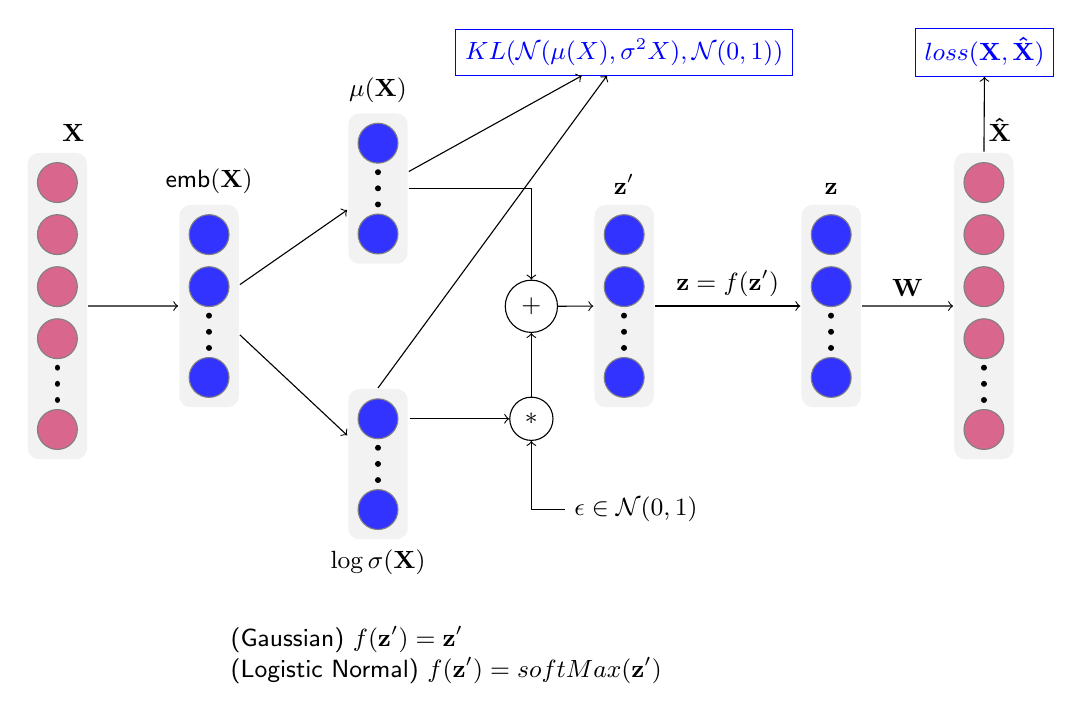
\begin{tikzpicture}[x={(1,0)},y={(0,1)},z={({cos(60)},{sin(60)})},
font=\sffamily\small,scale=2]

\node[circle,draw,gray,fill=purple!60] (A1) at (0,0,0) {~~~};
\node[circle,draw,gray,fill=purple!60,below=4pt of A1] (A2) {~~~};
\node[circle,draw,gray,fill=purple!60,below=4pt of A2] (A3) {~~~};
\node[circle,draw,gray,fill=purple!60,below=4pt of A3] (A4) {~~~};
\node[circle,draw,gray,fill=purple!60,below=18pt of A4] (A5) {~~~};
\draw[circle dotted, line width=2pt,shorten <=3pt] (A4) -- (A5);

\node[circle,draw,gray,fill=blue!80,right=40pt of A2] (E1) {~~~};
\node[circle,draw,gray,fill=blue!80,below=4pt of E1] (E2) {~~~};
\node[circle,draw,gray,fill=blue!80,below=18pt of E2] (E3) {~~~};
\draw[circle dotted, line width=2pt,shorten <=3pt] (E2) -- (E3);

\node[circle,draw,gray,fill=blue!80,right=80pt] (B1) at (0.5,0.25) {~~~};
\node[circle,draw,gray,fill=blue!80,below=18pt of B1] (B2) {~~~};
\draw[circle dotted, line width=2pt,shorten <=3pt] (B1) -- (B2);

\node[circle,draw,gray,fill=blue!80,right=80pt] (D1) at (0.5,-1.5) {~~~};
\node[circle,draw,gray,fill=blue!80,below=18pt of D1] (D2) {~~~};
\draw[circle dotted, line width=2pt,shorten <=3pt] (D1) -- (D2);

\node[circle,draw,gray,fill=blue!80,right=190pt of A2] (Z'1) {~~~};
\node[circle,draw,gray,fill=blue!80,below=4pt of Z'1] (Z'2) {~~~};
\node[circle,draw,gray,fill=blue!80,below=18pt of Z'2] (Z'3) {~~~};
\draw[circle dotted, line width=2pt,shorten <=3pt] (Z'2) -- (Z'3);

\node[circle,draw,gray,fill=blue!80,right=60pt of Z'1] (Z1) {~~~};
\node[circle,draw,gray,fill=blue!80,below=4pt of Z1] (Z2) {~~~};
\node[circle,draw,gray,fill=blue!80,below=18pt of Z2] (Z3) {~~~};
\draw[circle dotted, line width=2pt,shorten <=3pt] (Z2) -- (Z3);


\node[circle,draw,gray,fill=purple!60, right=320pt of A1] (C1) {~~~};
\node[circle,draw,gray,fill=purple!60, below=4pt of C1] (C2) {~~~};
\node[circle,draw,gray,fill=purple!60, below=4pt of C2] (C3) {~~~};
\node[circle,draw,gray,fill=purple!60, below=4pt of C3] (C4) {~~~};
\node[circle,draw,gray,fill=purple!60, below=18pt of C4] (C5) {~~~};
\draw[circle dotted, line width=2pt,shorten <=3pt] (C4) -- (C5);


\begin{scope}[on background layer]
\node[label={[xshift=.2cm]${\bf X}$},gray,thick,rounded corners,fill=gray!10,fit=(A1) (A5)] (AA1) {};
\node[label={${\bf \mu(X)}$},gray,thick,rounded corners,fill=gray!10,fit=(B1) (B2)] (BB1) {};
\node[label=below:{${\bf \log\sigma(X)}$},gray,thick,rounded corners,fill=gray!10,fit=(D1) (D2)] (DD1) {};
\node[label={[xshift=.2cm]${\bf {\hat{X}}}$},gray,thick,rounded corners,fill=gray!10,fit=(C1) (C5)] (CC1) {};
\node[label={emb$({\bf X})$},gray,thick,rounded corners,fill=gray!10,fit=(E1) (E3)] (EE1) {};
\node[label={${\bf z'}$},gray,thick,rounded corners,fill=gray!10,fit=(Z'1) (Z'3)] (ZZ'1) {};
\node[label={${\bf z}$},gray,thick,rounded corners,fill=gray!10,fit=(Z1) (Z3)] (ZZ1) {};
\end{scope}

\node[circle,draw,black,right=40pt of D1] (P1) {${\bf *}$};
\node[text width=3cm, right=60pt of D2] (EPS) {$\epsilon \in \mathcal{N}(0,1)$};
\node[circle,draw,black,above=23pt of P1] (P2) {${\bf +}$};

\node[rectangle,draw,blue,above=50pt of Z'1] (L2) {$KL(\mathcal{N}(\mu(X),\sigma^2{X}),\mathcal{N}(0,1))$};
\node[rectangle,draw,blue,right=44pt of L2] (L1) {$loss({\bf X},{\bf \hat{X}})$};

%\foreach \X in {1,2,3}
%{\draw[-latex] (A\X) -- (B2);}
%\draw[->] (AA1) -- (EE1) node[midway,above] {$q({\bf h}|{\bf X})$};
%\draw[->] (EE1) -- (CC1) node[midway,above] {$p({\bf \hat{X}}|{\bf h})$};
\draw[->] (AA1) -- (EE1) {};
\draw[->] (EE1) -- (BB1) {};
\draw[->] (EE1) -- (DD1) {};
\draw[->] (BB1) -| (P2) {};
\draw[->] (EPS) -| (P1) {};
\draw[->] (P1) -- (P2) {};
\draw[->] (D1) ++(0.2,0) -- (P1) {};
\draw[->] (P2) -- (ZZ'1) {};
\draw[->] (ZZ'1) -- (ZZ1) node[midway,above] {${\bf z} = f({\bf z'})$};
\draw[->] (ZZ1) -- (CC1) node[midway,above] {${\bf W}$};
\draw[->] (BB1) -- (L2) {};
\draw[->] (DD1.north) -- (L2) {};
\draw[->] (CC1.north) -- (L1) {};

\node[text width=10cm] at (3.6,-3) 
    {(Gaussian) $f({\bf z'}) = {\bf z'}$  \\ (Logistic Normal) $f({\bf z'}) = softMax({\bf z'})$};
  
\end{tikzpicture}



\end{document}
